\documentclass[a4paper,12pt]{article}
\usepackage[utf8]{vietnam}
\usepackage{fullpage}
\usepackage{amsmath,amsxtra,amssymb,amsthm,latexsy m,amscd,amsfonts}
\usepackage{graphicx}
\begin{document}
\centerline{\textbf{\large{LẬP LỊCH CÁC CÔNG VIỆC CÓ CHU KỲ}}}
\centerline{\textbf{\large{VÀ KHÔNG CHU KỲ TRONG MÔI TRƯỜNG}}}
\centerline{\textbf{\large{MÁY ĐƠN ĐỂ TỐI ƯU HÓA ĐA MỤC TIÊU}}}
\centerline{\textbf{\large{THỜI GIAN HOÀN THÀNH VÀ TỔNG ĐỘ TRỄ}}}
\tableofcontents
\newpage
\section{Tóm lược}
Nhiều ứng dụng điều khiển yêu cầu cả 2 kiểu công việc, có chu kỳ (periodic) và không có chu kỳ (aperiodic). Hai kiểu công việc này khác nhau về mức độ quan trọng. Các công việc có chu kỳ thông thường có ràng buộc cứng về kì hạn (deadline) trong khi các công việc không có chu kỳ thường có kì hạn mềm hoặc có thể không có kì hạn. Trong báo cáo này chúng ta giới thiệu và giải quyết vấn đề lập lịch trong môi trường máy đơn bao gồm các công việc có chu kỳ và không có chu kỳ. Mục tiêu của quá trình lâp lịch là tối ưu hóa đa mục tiêu bao gồm 2 mục tiêu là: thời gian hoàn thành (makespan) và tổng độ trễ (total tardiness) của các công việc không có chu kỳ trong khi vẫn đảm bảo ràng buộc về thời gian của tất cả các công việc có chu kỳ. Trong khi lập lịch đồng thời 2 mục tiêu trên chúng ta cần phải đảm bảo sự cân bằng về yêu cầu, trọng số của 2 mục tiêu. Đầu tiên chúng ta sẽ chứng minh rằng vấn đề đã nêu có độ khó là NP-Hard và sau đó sẽ giới thiệu một giải thuật heuristic tích hợp được mở rộng, tiến triển từ thứ tự LPT cổ điển (Longest Processing Time) cho việc lập lịch đối ưu mục tiêu makespan và thứ tự EDF cổ điển (Earliest Deadline First) cho việc lập lịch tối ưu mục tiêu tổng độ trễ (total tardiness). Hiệu suất của giải thuật được đề xuất sẽ được đánh giá thông qua các kết quả thực nghiệm.
\section{Giới thiệu}
Trong nhiều ứng dụng điều khiển thời gian thực, các công việc có chu kỳ yêu cầu các nhu cầu tính toán chính trong hệ thống. Các công việc có chu kỳ thông thường tạo ra bởi các quá trình quan sát và thu thập dữ liệu, kiểm soát vòng lặp, lên kế hoạch và quản lý hệ thống. Các công việc như thế cần phải được thực thi một cách có chu kỳ theo một tỷ lệ nhất định được dẫn xuất từ các yêu cầu của ứng dụng. Công việc có chu kỳ được thực thi chính xác một lần trong chu kỳ của công việc đó. Các công việc không có chu kỳ là các công việc mà tần số xuất hiện là không bị ràng buộc. Các công việc không có chu kỳ được phân bố và thực thi một cách ngẫu nhiên, ví dụ tuân theo phân bố Poisson và không thể có các kì hạn cứng.\\\\
Trong bài báo này, chúng ta xem xét vấn đề lập lịch trong môi trường máy đơn được mô tả như sau: cho một tập hợp $N$ bao gồm $n$ các công việc độc lập không thể bắt đầu lại (non-resume) $J = \{J_1, J_2,\ldots,J_n\}$ với các thời gian xử lý $p_i, 1 \le i \le n$ và tập các deadline $d_i, 1 \le i \le n$. Ở đây không thể bắt đầu lại có nghĩa là một công việc nếu không thể hoàn thành trước công việc bảo trì, nó phải được bắt đầu lại. Tất cả các công việc có thể bắt đầu tại thời điểm $0$. Thời gian thực thi của các công việc có chu kỳ (mỗi công việc bảo trì) là $p$. Cho rằng độ dài khoảng thời gian giữa 2 công việc có chu kỳ là $T$. $T_k$ là chu kỳ thứ $k$ tương ứng với công việc có chu kỳ. Chúng ta có thể thấy rằng $p_i \le 2(T-p)$, ngược lại sẽ không thể có được một lịch biểu hợp lệ vì sẽ có một chu kỳ mà không thể có công việc có chu kỳ nào được thực thi.\\\\
Mục tiêu của bài toán là tối thiểu hóa đồng thời 2 mục tiêu là $C_{max}$ -  thời gian hoàn thành; và $\sum T_i$ -  tổng độ trễ của các công việc không có chu kỳ trong tập $N$. Tương ứng với các ký hiệu trong bài toán lập lịch, bài toán lập lịch trên có thể được kí hiệu như sau $\mathbf{1 | \mbox{\textbf{periodic job}} (c,p), \mbox{\textbf{aperiodic job set}} (N) |  C_{max}(N), \sum T_i}$.\\\\
Đóng góp chính của báo cáo này bao gồm việc chứng minh NP-Hard cho vấn đề lập lịch được xem xét ở trên và cung cấp một heuristic tích hợp đồng thời cho thứ tự LPT cổ điển (Longest Processing Time) và EDF cổ điển (Earliest Deadline First).\\\\
Phần còn lại của báo cáo được tổ chức như sau. Phần 3 sẽ chứng minh bài toán có độ khó là NP-Hard. Phần 4 cung cấp chi tiết của heuristic đề xuất. Phần 5 thảo luận các kết quả thực nghiệm để xem xét hiệu suất của heuristic. Phần 6 bao gồm kết luận của báo cáo và các thảo luận các công việc trong tương lai.
\section{Bài toán NP-Hard}
\section{Heuristic đề xuất}
\subsection{Heuristic cho thứ tự LPT}
Ý tưởng của heuristic được đưa ra dựa vào việc phân tích trường hợp xấu nhất của giải thuật LPT. Trong giải thuật LPT, chúng ta sẽ sắp xếp các công việc không có chu kỳ theo thứ tự giảm dần thời gian xử lý, nếu 2 công việc có cùng thời gian xử lý thì chúng ta sẽ sắp xếp công việc có deadline nhỏ hơn ở phía trước. Ví dụ đầu vào dữ liệu sau đây.

\begin{itemize}
\item
$N = \{1, 2, 3, 4, 5, 6, 7, 8, 9, 10\}$ với $P = \{15, 12, 9, 6, 1, 7, 8, 9, 13, 16\}$ và\\ $D = \{16, 42, 50, 25, 70, 75, 40, 90, 25, 80\}$
\item
$T = 10, p = 1$
\end{itemize}

Sau khi sắp xếp theo thứ tự LPT nêu ra ở trên thì thứ tự công việc như sau:\\\\
\begin{tabular}{|c|c|c|c|c|c|c|c|c|c|c|}
\hline
Công việc&10&1&9&2&3&8&7&6&4&5\\
\hline
Thời gian xử lý&16&15&13&12&9&9&8&7&6&1\\
\hline
Deadline&80&16&25&42&50&90&40&75&25&70\\
\hline
\end{tabular}
\\\\\\
Lịch biểu kết quả khi chạy giải thuật LPT (màu đỏ biểu diễn cho công việc không có chu kỳ, màu xanh biểu diễn cho công việc có chu kỳ):
\begin{center}
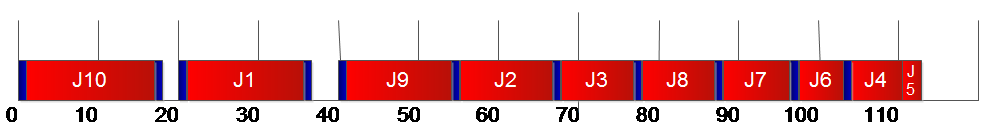
\includegraphics[scale=0.65]{Fig_1.png}
\\
Hình 1: Một lịch biểu tạo ra bởi giải thuật LPT.
\end{center}

Dựa theo thứ tự LPT, $C_{max}(N) = 112$ (theo hình 1) và có 3 đơn vị thời gian rảnh (tương ứng với khoảng thời gian [18, 20]). Tồn tại khoảng thời gian rỗi này bởi vì công việc $J_2$ không thể bắt đầu tại thời điểm 17 và không có công việc có chu kỳ nào có thể thực thi tại giai đoạn thứ 3.\\\\
Để khắc phục sự bất tiện này, chúng ta cung cấp một chiến lược để sửa đổi giải thuật LPT: \textit{tại bất kỳ thời điểm $t$ nào khi một công việc được xem xét $J_k$ (theo thứ tự LPT) không thể được bắt đầu (ngược lại, sẽ tạo ra thời gian rổi), chúng ta tìm công việc khác để thực thi tại thời điểm này.} Chiến lược được đưa ra như sau:\\\\
\textbf{Heuristic HEU1}: \textit{Công việc có thời gian xử lý lâu nhất trong số các công việc có thể bắt đầu tại thời điểm $t$ (và không tạo ra thêm bất kỳ thời gian rỗi nào tại thời điểm $t$)}.\\\\
Dựa vào lịch biểu ở hình 1, với heuristic HEU1 trên chúng ta có các kết quả như sau. HEU1 có \textit{makespan là 106} (xem hình 2).
\begin{center}
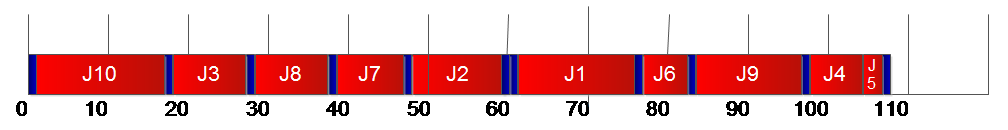
\includegraphics[scale=0.65]{Fig_2.png}
\\
Hình 2: Một lịch biểu tạo ra bởi giải thuật LPT với HEU1.
\end{center}
\subsection{Heuristic cho thứ tự EDF}
Ý tưởng của heuristic được đưa ra dựa vào việc phân tích trường hợp xấu nhất của giải thuật EDF. Trong giải thuật EDF, chúng ta sẽ sắp xếp các công việc không có chu kỳ theo thứ tự tăng dần của deadline, nếu 2 công việc có cùng deadline thì chúng ta sẽ sắp xếp công việc có thời gian xử lý dài hơn ở phía trước. Ví dụ đầu vào dữ liệu sau đây.

\begin{itemize}
\item
$N = \{1, 2, 3, 4, 5, 6, 7, 8, 9, 10\}$ với $P = \{15, 12, 9, 6, 1, 7, 8, 9, 13, 16\}$ và\\ $D = \{16, 42, 50, 25, 70, 75, 40, 90, 25, 80\}$
\item
$T = 10, p = 1$
\end{itemize}

Sau khi sắp xếp theo thứ tự EDF nêu ra ở trên thì thứ tự công việc như sau:\\\\
\begin{tabular}{|c|c|c|c|c|c|c|c|c|c|c|}
\hline
Công việc&1&9&4&7&2&3&5&6&10&8\\
\hline
Deadline&16&25&25&40&42&50&70&75&80&90\\
\hline
Thời gian xử lý&15&13&6&8&12&9&1&7&16&9\\
\hline
\end{tabular}
\\\\\\
Lịch biểu kết quả khi chạy giải thuật EDF (màu đỏ biểu diễn cho công việc không có chu kỳ, màu xanh biểu diễn cho công việc có chu kỳ):
\begin{center}
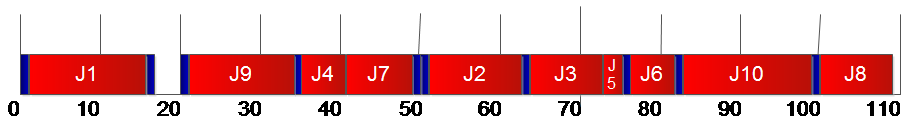
\includegraphics[scale=0.7]{Fig_3.png}
\\
Hình 3: Một lịch biểu tạo ra bởi giải thuật EDF.
\end{center}
Dựa vào lịch biểu trên thì chúng ta có thể tính toán được tổng độ trễ của lịch biểu:
\[
\sum T_i = \sum max(0, C_i - d_i) = 127
\]
Dựa theo thứ tự EDF, $\sum T_i = 127$ (theo hình 3) và có 3 đơn vị thời gian rảnh (tương ứng với khoảng thời gian [18, 20]). Tồn tại khoảng thời gian rỗi này bởi vì công việc $J_9$ không thể bắt đầu tại thời điểm 17 và không có công việc có chu kỳ nào có thể thực thi tại giai đoạn thứ 3.\\\\
Để khắc phục sự bất tiện này, chúng ta cung cấp một chiến lược để sửa đổi giải thuật EDEF: \textit{tại bất kỳ thời điểm $t$ nào khi một công việc được xem xét $J_k$ (theo thứ tự EDF) không thể được bắt đầu (ngược lại, sẽ tạo ra thời gian rổi), chúng ta tìm công việc khác để thực thi tại thời điểm này.} Chiến lược lựa chọn công việc thực thi như sau:\\\\
\textbf{Heuristic HEU2}: \textit{Lựa chọn công việc có deadline nhỏ nhất trong số các công việc có thể bắt đầu tại thời điểm $t$ (và không tạo ra bất kỳ thời gian rỗi nào tại thời điểm $t$).}\\\\
Dựa vào lịch biểu ở hình 3 áp dụng HEU2 chúng ta có được lịch biểu như sau với \textit{tổng độ trễ là 85}.
\begin{center}
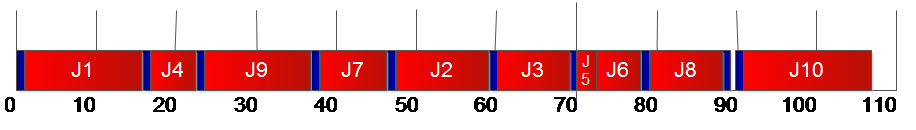
\includegraphics[scale=0.7]{Fig_4.png}
\\
Hình 4: Một lịch biểu tạo ra bởi giải thuật EDF với heuristic HEU2.
\end{center}
\subsection{Kết hợp heuristic để tối ưu đồng thời 2 mục tiêu}
Chúng ta đã giới thiệu 2 heuristic để tối ưu 2 mục tiêu riêng lẽ là thời gian hoàn thành và tổng độ trễ. Trong từng trường hợp tối ưu, chúng ta chỉ tối ưu 1 mục tiêu riêng lẽ mà không quan tâm đến mục tiêu còn lại. Trong quá trình tối ưu mục tiêu makespan với heuristic HEU1 chúng ta có được makespan tốt là \textit{106} nhưng tổng độ trễ của lịch biểu không tốt là $\sum T_i = 281$. Tương tự cho trường hợp sử dụng heuristic HEU2 chúng ta đạt được tổng độ trễ là $\sum T_i = 85$ nhưng makespan đạt được là \textit{107}. Trong phần này chúng ta sẽ kết hợp 2 heuristic HEU1 và HEU2 một cách đồng thời để cân bằng về độ tốt của cả 2 mục tiêu là makespan và tổng độ trễ.\\\\
Ý tưởng kết hợp 2 mục tiêu như sau:
\begin{itemize}
\item
Đầu tiên chúng ta sẽ sắp xếp các công việc theo thứ tự LPT và thứ tự EDF. Như vậy chúng ta sẽ có 2 tập các công việc có thứ tự khác nhau là LPT (tập $J_{LPT}$) và EDF (tập $J_{EDF}$).
\item
2 mục tiêu sẽ có độ ưu tiên (Priority Degree) khác nhau là $D_{LPT}$ và $D_{EDF}$, trong từng bước lập lịch một công việc chúng ta sẽ xem xét lập lịch cho mục tiêu có độ ưu tiên cao hơn. Sau khi một công việc đã được lập lịch cho một mục tiêu thì độ ưu tiên của mục tiêu đó sẽ giảm đi và tiếp theo chúng ta lại xem xét độ ưu tiên giữa 2 mục tiêu để lựa chọn mục tiêu sẽ được lập lịch tiếp theo.
\item
Dựa vào mục tiêu được lựa chọn để lập lịch chúng ta sẽ quyết định sử dụng heuristic nào, HEU1 hay HEU2, sử dụng tập công việc theo thứ tự LPT hay EDF để lập lịch. Khi một công việc của tập LPT được lập lịch thì đồng thời chúng ta cũng loại bỏ công việc đó đi trong tập EDF, và ngược lại.
\item
Cuối cùng là vấn đề đánh giá độ ưu tiên của 2 mục tiêu như thế nào. Chúng ta sẽ có 2 tham số $\alpha$ và $\beta$ gọi là hệ số độ ưu tiên cho 2 mục tiêu makespan và tổng độ trễ. Công thức tính độ ưu tiên như sau sẽ là:\textit{ Độ ưu tiên = Hệ số ưu tiên * (Số công việc chưa được lập lịch - Số công việc đã lập lịch của tập thứ tự)}
\end{itemize}
Áp dụng cho trường hợp dữ liệu đầu vào ở trên:
\begin{itemize}
\item
$N = \{1, 2, 3, 4, 5, 6, 7, 8, 9, 10\}$ với $P = \{15, 12, 9, 6, 1, 7, 8, 9, 13, 16\}$ và\\ $D = \{16, 42, 50, 25, 70, 75, 40, 90, 25, 80\}$
\item
$T = 10, p = 1$
\end{itemize}
Tập công việc có thứ tự LPT ($J_{LPT}$):\\\\
\begin{tabular}{|c|c|c|c|c|c|c|c|c|c|c|}
\hline
Công việc&10&1&9&2&3&8&7&6&4&5\\
\hline
Thời gian xử lý&16&15&13&12&9&9&8&7&6&1\\
\hline
Deadline&80&16&25&42&50&90&40&75&25&70\\
\hline
\end{tabular}
\\\\\\
Tập công việc có thứ tự EDF ($J_{EDF}$):\\\\
\begin{tabular}{|c|c|c|c|c|c|c|c|c|c|c|}
\hline
Công việc&1&9&4&7&2&3&5&6&10&8\\
\hline
Deadline&16&25&25&40&42&50&70&75&80&90\\
\hline
Thời gian xử lý&15&13&6&8&12&9&1&7&16&9\\
\hline
\end{tabular}
\\\\\\
Với hệ số ưu tiên của mục tiêu makespan $\alpha = 0.6$ và mục tiêu tổng độ trễ là $\beta = 0.4$. Vì chưa có công việc nào được lập lịch nên độ ưu tiên của makespan là $D_{LPT} = 0.6*(10 - 0) = 6$ và của mục tiêu tổng độ trễ là $D_{EDF} = 0.4*(10 - 0) = 4$. Vì $D_{LPT} > D_{EDF}$ nên công việc đầu tiên sẽ lập lịch theo mục tiêu makespan, là công việc trong tập $J_{LPT}$ với \textbf{số thứ tự = 10, thời gian xử lý = 16, deadline = 80} do sử dụng \textbf{heuristic HEU1}. Sau khi lập lịch công việc, chúng ta sẽ xóa công việc này ra khỏi tập thứ tự LPT và EDF.\\\\
Sau đó độ ưu tiên được cập nhật $D_{LPT} = 0.6*(9 - 1) = 4.8$ và $D_{EDF} = 0.4*(9 - 0) = 3.6$, vì $D_{LPT} > D_{EDF}$ nên công việc tiếp theo sẽ lập lịch theo mục tiêu makespan là công việc trong tập $J_{LPT}$ với \textbf{số thứ tự = 3, thời gian xử lý = 9, deadline = 50} do sử dụng \textbf{heuristic HEU1}. Sau khi lập lịch công việc, chúng ta sẽ xóa công việc này ra khỏi tập thứ tự LPT và EDF.\\\\
Sau đó độ ưu tiên được cập nhật $D_{LPT} = 0.6*(8 - 2) = 3.6$ và $D_{EDF} = 0.4*(8 - 0) = 3.2$, vì $D_{LPT} > D_{EDF}$ nên công việc tiếp theo sẽ lập lịch theo mục tiêu makespan là công việc trong tập $J_{LPT}$ với \textbf{số thứ tự = 8, thời gian xử lý = 9, deadline = 90} do sử dụng \textbf{heuristic HEU1}. Sau khi lập lịch công việc, chúng ta sẽ xóa công việc này ra khỏi tập thứ tự LPT và EDF.\\\\
Sau đó độ ưu tiên được cập nhật $D_{LPT} = 0.6*(7 - 3) = 2.4$ và $D_{EDF} = 0.4*(7 - 0) = 2.8$, vì $D_{LPT} < D_{EDF}$ nên công việc tiếp theo sẽ lập lịch theo mục tiêu tổng độ trễ là công việc trong tập $J_{EDF}$ với \textbf{số thứ tự = 4, thời gian xử lý = 6, deadline = 25} do sử dụng \textbf{heuristic HEU2}. Sau khi lập lịch công việc, chúng ta sẽ xóa công việc này ra khỏi tập thứ tự EDF và LPT.\\\\
Tiếp tục cho đến khi tất cả công việc được lập lịch, chúng ta có lịch biểu cuối cùng như sau:
\begin{center}
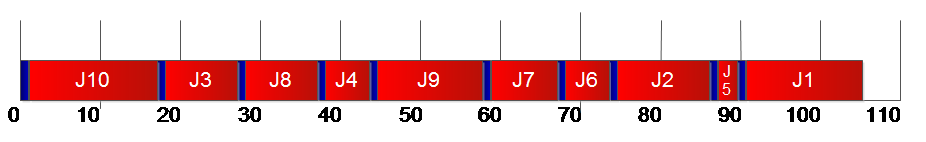
\includegraphics[scale=0.7]{Fig_5.png}
\\
Hình 5: Một lịch biểu tạo ra bởi kết hợp 2 heuristic HEU1 và HEU2.
\end{center}
Lịch biểu kết quả này có \textit{makespan là 106} bằng với HEU1 là 106 nhưng nhỏ hơn so với HEU2 là 107 và có \textit{tổng độ trễ là 235} nhỏ hơn so với HEU1 là 281 và lớn hơn so với HEU2 là 85. Đây có thể là một lịch biểu khả thi để cân bằng 2 mục tiêu makespan và tổng độ trễ khi lập lịch với dữ liệu đầu vào ở trên.
\section{Kết quả thực nghiệm}
Trong phần này, chúng ta sẽ xem xét hiệu suất của việc kết hợp 2 heuristic HEU1 và HEU2 so với sử dụng từng heuristic khi lập lịch. Phần cứng sử dụng cho thực nghiệm bao gồm CPU Intel R Corei5 với 2MB cache L2, tốc độ tính toán 2.53GHz, bộ nhớ 3GB DDR2 SDRAM. Đầu vào của mỗi lần chạy bao gồm chu kỳ của quá trình, thời gian xử lý của công việc có chu kỳ, số lượng công việc không có chu kỳ và thời gian xử lý của mỗi công việc không có chu kỳ được tạo một cách ngẫu nhiên nhưng giá trị lớn nhất không được vượt quá $2*(cycle-\mbox{periodic processing time})$ để có thể tạo được lịch biểu khả thi. Tập dữ liệu đầu vào cho chu kỳ $C = \{90,100\}$, thời gian xử lý công việc có chu kỳ $P = \{40,50\}$ và số lượng công việc không chu kỳ $N = \{100,1000\}$, và các hệ số ưu tiên cho makespan là $\alpha = 0.6$ và cho tổng độ trễ là $\beta = 0.4$. Kết quả thực nghiệm được cho bởi bảng 1 sau.\\
\begin{center}
\begin{tabular}{|c|c|c|c|c|c|c|c|c|c|c|}
\hline
Cycle&Periodic&Aperiodic&LPTCmax&LPTTar&EDFCmax&EDFTar&Cmax&Tardiness\\
\hline
90&40&100&8733&319320&8852&164775&8762&248367\\
\hline
90&40&1000&89751&35427070&90668&17642817&89791&28893954\\
\hline
90&50&100&9275&384599&9399&219027&9275&323240\\
\hline
90&50&1000&89589&39157821&90122&23684233&89639&33660225\\
\hline
100&40&100&8137&298433&8146&124571&8177&253132\\
\hline
100&40&1000&99653&36179588&100257&17100526&99693&28934685\\
\hline
100&50&100&10339&400902&10626&210004&10339&339978\\
\hline
100&50&1000&99036&40517203&99841&21850027&99036&33004695\\
\hline
\end{tabular}
\end{center}
\begin{itemize}
\item
\textit{Cycle:} Chu kỳ của công việc có chu kỳ.
\item
\textit{Periodic:} Thời gian tính toán của công việc có chu kỳ.
\item
\textit{Aperiodic:} Số lượng các công việc không có chu kỳ.
\item
\textit{LPTCmax:} Thời gian hoàn thành khi sử dụng riêng rẽ HEU1.
\item
\textit{LPTTar:} Tổng độ trễ khi sử dụng riêng rẽ HEU1.
\item
\textit{EDFCmax:} Thời gian hoàn thành khi sử dụng riêng rẽ HEU2.
\item
\textit{EDFTar:} Tổng độ trễ khi sử dụng riêng rẽ HEU2.
\item
\textit{Cmax:} Thời gian hoàn thành khi sử dụng kết hợp HEU1 và HEU2.
\item
\textit{Tardiness:} Tổng độ trễ khi sử dụng kết hợp HEU1 và HEU2.
\end{itemize}
\begin{center}
Bảng 1: Kết quả thực nghiệm.\\
\end{center}
\section{Kết luận}
Trong báo cáo này, chúng ta đã xem xét vấn đề lập lịch trong môi trường máy đơn với 2 loại công việc có chu kỳ và không có chu kỳ. Mục tiêu của quá trình là đảm bảo về sự cân bằng giữa 2 mục tiêu thời gian hoàn thành và tổng độ trễ của các công việc không có chu kỳ trong khi vẫn đảm bảo ràng buộc về kì hạn của các công việc có chu kỳ trong mỗi chu kỳ thời gian. Chúng ta đã chứng minh rằng bài toán này thuộc lớp NP-Hard. Sau đó, chúng ta đề xuất một heuristic tích hợp cải tiến thứ tự LPT cổ điển và EDF cổ điển. Các kết quả thực nghiệm chứng tỏ rằng hiệu suất của heuristic kết hợp này cho ra được kết quả cân bằng giữa 2 mục tiêu thời gian hoàn thành và tổng độ trễ, không quá chú trọng vào mục tiêu thời gian hoàn thành mà bỏ qua mục tiêu tổng độ trễ và ngược lại.\\\\
Xem xét bài toán này có thể dẫn đến việc xem xét và nghiên cứu những vấn đề nghiên cứu mở rộng hơn nữa. Mục tiêu có thể là tối thiểu hóa không chỉ là tổng độ trễ mà còn có thể là độ trễ tối đa, số lượng các công việc bị trễ, ... Các giải thuật heuristic xấp xỉ và chính xác có thể được xem xét để giải quyết vấn đề lập lịch này trong tương lai. Đồng thời chúng ta có thể xem xét bài toán tối ưu đa mục tiêu trong tương lai, ví dụ như kết hợp 2 mục tiêu khác ngoài makespan và tổng độ trễ, hoặc nhiều hơn 2 mục tiêu trong cùng một bài toán lập lịch máy đơn cho các công việc có chu kỳ và công việc không có chu kỳ.
\section{Tài liệu tham khảo}
1.	M.R. Garey, D.S. Johnson. Computers and Intractability: A Guide to the Theory of NP-Completeness. W.H. Freeman \& Company, San Francisco, 1979.\\
2.	R.L. Graham, E.L. Lawler, J.K. Lenstra, and A.H.G. Rinnooy Kan. Optimization and approximation in deterministic sequencing and scheduling: a survey. Annals of Discrete Mathematics 5, pp. 287–326, 1979.\\
3.	M. Ji, Y. He, T.C.E. Cheng. Single-machine scheduling with periodic maintenance to minimize makespan. Computer \& Operations Research 34, pp. 1764-1770, 2007.\\
4.	C.J. Liao, W.J. Chen. Single-machine scheduling with periodic maintenance and non-resumable jobs.
\end{document}